\documentclass[aspectratio=43]{beamer}
\usepackage[utf8]{inputenc}
\usepackage{multicol}

%% Useful packages
\usepackage{amsmath}
\usepackage{graphicx}
\graphicspath{{fig/}}
\usepackage{xcolor}
\usepackage{tikz}

\newcommand{\height}{H}
\newcommand{\av}[1]{\langle {#1} \rangle}
\newcommand{\vect}[1]{\mathbf{#1}}


\title{3D-PTV with FPGA for Lagrangian measurements in a wind tunnel}
\date{July 9, 2018}
\author[Liberzon]{Alex Liberzon, Tel Aviv University}


\usetheme{material}

\useDarkTheme
%\useLightTheme
\usePrimaryRed
\useAccentGreen


\begin{document}




\begin{frame}
\titlepage
\end{frame}

\begin{frame}{Tel Aviv University \href{http://www.youtube.com/watch?v=rbUevEuYQHg}{ ...  promotional video}}
\begin{multicols}{2}
\centering
\cardImg{telaviv}{.48\textwidth} \cardImg{sculpture_tau_polymer}{0.48\textwidth}
\cardImg{telaviv2}{.48\textwidth}\cardImg{wolfson}{0.48\textwidth}
\end{multicols}
\end{frame}
%
%%\end{frontmatter}
\begin{frame}{take-home message}
\begin{itemize}
\item Real-time image analysis on a dedicated hardware is implemented for long-recording, high speed 3D-PTV
\item This extension changes few paradigms about 3D-PTV from in-lab table-top experiments to wind tunnel and field experiments
\item Unprecedented data set of millions of tracer trajectories recorded in a canopy flow model in an environmental wind tunnel, providing Lagrangian velocity and acceleration distributions in an urban canopy flow model
\end{itemize}

\begin{cardTiny}\href{https://arxiv.org/abs/1806.04975}{Details are in the pre-print ``Real-time extension ...'' by Shnapp et al.  arXiv:1806.04975}
\end{cardTiny}

\end{frame}
%
\section{Introduction}
\begin{frame}{The credit goes to ... }
\begin{multicols}{2}
\centering
\cardImg{group_photo.jpg}{.49\textwidth} \cardImg{calibration_team.jpg}{0.49\textwidth}
\cardImg{sabrina_caliper.jpg}{.49\textwidth}\cardImg{meny_sabrina.jpg}{0.49\textwidth}
\end{multicols}
\end{frame}
%
\begin{frame}
\begin{card}[Israeli Institute for Biological Research]
Eyal Fattal, Yardena Raviv, Valery Babin, Mordechai Hotoveli, David Perry
\end{card}
\begin{card}[TAU]
Ron Shnapp, Meny Kon, Grigori Gulitski, Sabrina Shlain
\end{card}
\begin{card}[Funding]
Israel Science Foundation, PAZY Grant, Metro 450 grant
\end{card}
\end{frame}
%
%\section{Introduction}
%
%\section{Three Dimensional Particle Tracking Velocimetry (3D-PTV)}
%
\begin{frame}{Let's follow the Lagrangian path}
\centering\cardImg{art}{0.8\textwidth}
\vspace{-.3cm}
\begin{cardTiny}
``Marianthe'' invited people inside turbulent forms to experience them as
if they were a particle borne along in the flow. Athena
Tacha (1985), \href{http://nautil.us/issue/15/turbulence/the-scientific-problem-that-must-be-experienced}{``Nautilus'' by Philip Ball}
\end{cardTiny}
\end{frame}
%



\begin{frame}{Quick intro to 3D-PTV}
\centering\cardImg{ptv-scheme}{1.0\textwidth}
\end{frame}

%
\begin{frame}{Basic steps}
\begin{columns}[t]
	\begin{column}{0.4\textwidth}
		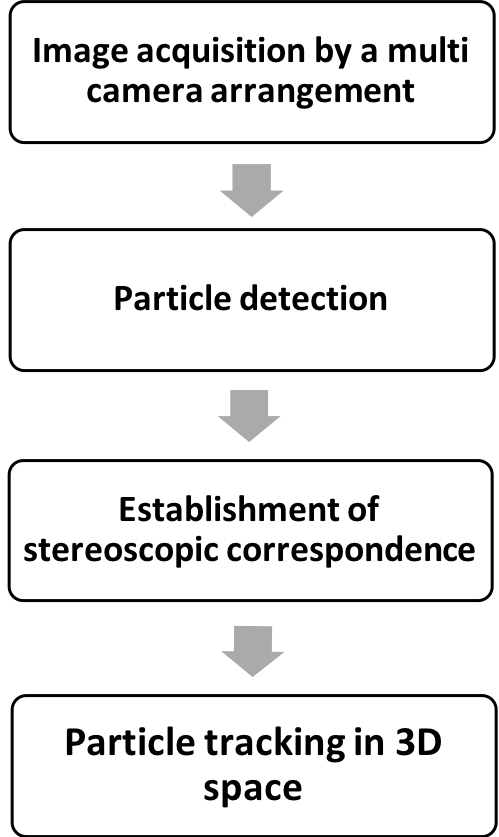
\includegraphics[height=.8\textheight]{ptv_blocks}
	\end{column}
	\begin{column}{0.3\textwidth}
		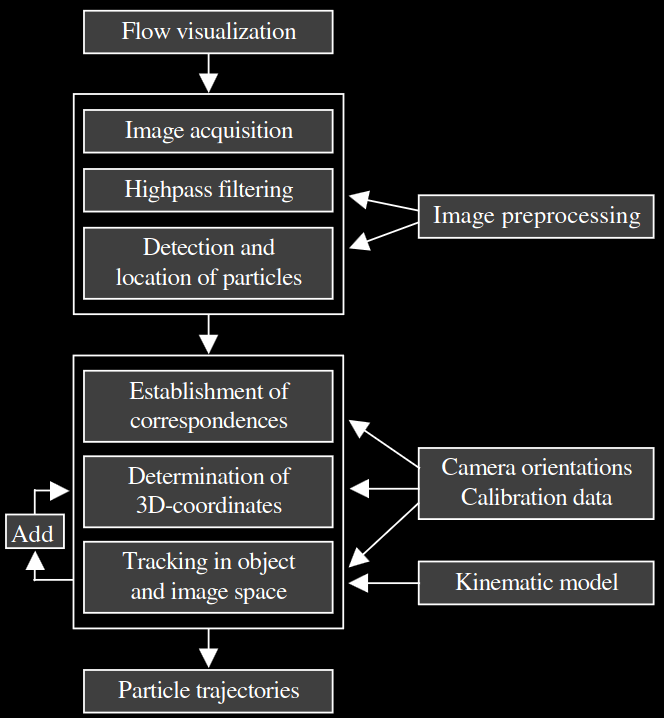
\includegraphics[height=.8\textheight]{ptv_steps}
	\end{column}
\end{columns}
\end{frame}


\begin{frame}{Epipolar geometry}
\begin{multicols}{2}
\cardImg{epipolar1}{.49\textwidth}
\cardImg{epipolar}{.49\textwidth}
\end{multicols}
\end{frame}

\begin{frame}{Tracking}
\centering\cardImg{tracking}{.9\textwidth}
\end{frame}

\begin{frame}{The immediate result is a Lagrangian trajectory}
\begin{multicols}{2}
\centering
\cardImg{moffatt1}{.49\textwidth}
\cardImg{particle_trajectories}{.49\textwidth}
\end{multicols}
\end{frame}


%\begin{frame}{Lagrangian to Eulerian post-processing}
%\centering\cardImg{voxel1}{.6\textwidth}
%\end{frame}
%
\begin{frame}{3D-PTV main focus is turbulence}
\begin{cardTiny} 
Which means we need  the \alert{full gradient tensor} along the particle trajectories:
$\partial u_{i}/\partial x_{j}$ in space and time
\end{cardTiny}

\begin{multicols}{2}
\centering
\cardImg{moffatt2}{.49\textwidth}
\cardImg{ptvgif}{.49\textwidth}
\end{multicols}
\end{frame}

\begin{frame}{It had other applications, e.g. inertial clustering}
\centering\cardImg{two_phase_3dptv}{.9\textwidth}
\end{frame}

\begin{frame}{MRI + 3D-PTV}
\begin{multicols}{2}
\centering
\cardImg{mri2}{.35\textwidth}
\cardImg{mri3}{.35\textwidth}
\end{multicols}
\centering\cardImg{mri1}{.5\textwidth}
\end{frame}


\begin{frame}{3D PTV is typically a lab system}
\centering\cardImg{lab.jpg}{.9\textwidth}
\end{frame}

\begin{frame}{The main bottleneck is also heavy}
\begin{multicols}{2}
\centering
\cardImg{ptv_drives1}{.49\textwidth}
\cardImg{ptv_drives2}{.49\textwidth}
\end{multicols}
\end{frame}


\begin{frame}{We had a dream: 3D-PTV for large scale systems}
\centering\cardImg{car_ptv.png}{.8\textwidth}
\end{frame}

% \subsubsection*{Real time image acquisition and processing}
%\begin{frame}{The solution}
%\begin{card}
%\end{card}
%\end{frame}


\begin{frame}{Need to eliminate the transfer rate bottleneck}
\begin{card}[from compression to on-camera processing]
\begin{multicols}{2}
\centering
\cardImg{realtime1}{.49\textwidth}
\cardImg{voth}{.48\textwidth}
\cardImg{mikrotron_sobel}{.49\textwidth}
\cardImg{mikrotron_inside}{.49\textwidth}
\end{multicols}
\end{card}
\end{frame}

\begin{frame}{Sobel edge detection based algorithm}
\centering
\cardImg{sobel_1}{.8\textwidth}
\end{frame}


\begin{frame}{Works very well for lab experiments}
\begin{card}
\centering
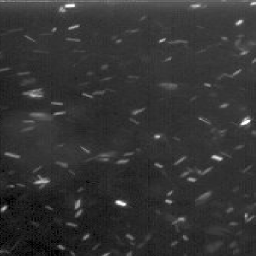
\includegraphics[width=.32\textwidth]{1_in}
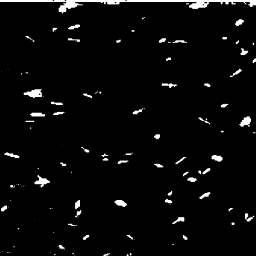
\includegraphics[width=.32\textwidth]{1_binarized}
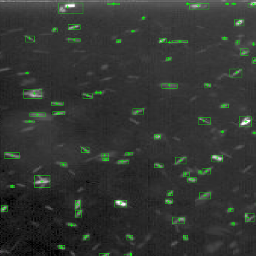
\includegraphics[width=.32\textwidth]{1_out}
\end{card}
\vspace{-.5cm}
\begin{cardTiny}
Raw image - binarized image - blobs marked on the original image.  
\end{cardTiny}
\end{frame}


\begin{frame}{Real life is not like this}
\begin{multicols}{2}
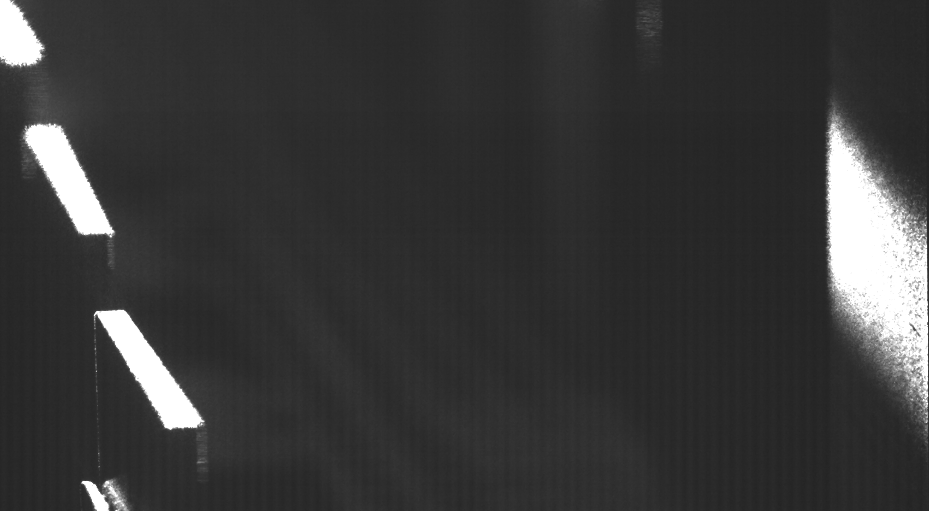
\includegraphics[width=.49\textwidth]{background.png}
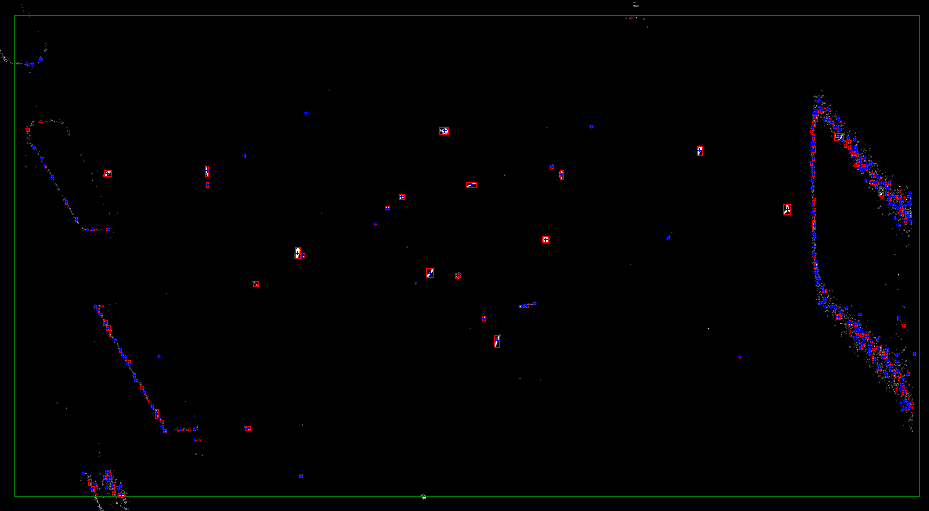
\includegraphics[width=.49\textwidth]{detection.png}
\end{multicols}
\begin{cardTiny}
Raw 3D-PTV image the wind tunnel experiments: Background ->  binary image after background subtraction, and detection using a local adaptive filter
\end{cardTiny}
\end{frame}

\begin{frame}{We had to develop the know-how}
\centering\cardImg{1vision_blob_recorder}{1\textwidth}
\end{frame}


\begin{frame}{Image processing algorithm on FPGA}
\centering\cardImg{blob_analysis.png}{1\textwidth}
% \begin{cardTiny} Diagram of the blob analysis algorithm. \end{cardTiny}
\end{frame}

\begin{frame}{And its implementation on a dedicated hardware}
\begin{multicols}{2}
\centering
\cardImg{1vision_blob_recorder_1}{.8\textwidth}
\cardImg{backside}{.25\textwidth}
\end{multicols}
\end{frame}


\begin{frame}{And now we are ready for the Environmental Wind Tunnel}
\cardImg{wind_tunnel_photo_1}{0.9\textwidth}
\end{frame}

\begin{frame}{Top view of the canopy model, systems locations}
\centering\cardImg{setup_drawing.png}{0.99\textwidth}
\end{frame}


\begin{frame}
\begin{multicols}{2}
\centering
\cardImg{camera_system_laser.jpg}{0.49\textwidth}
\cardImg{calibration_in_laser.jpg}{.49\textwidth}
\end{multicols}
\begin{cardTiny}
Four cameras pointing into the measurement location as seen from the test section inside the tunnel, and the calibration target mounted on the traverse arm.
\end{cardTiny}
\end{frame}

%
%\begin{frame}
%\begin{multicols}{2}
%\centering\cardImg{img1.jpg}{.49\textwidth}
%\cardImg{camera_system_laser.jpg}{0.49\textwidth}
%\end{multicols}
%\end{frame}

\begin{frame}{Pressurized air seeding devices}
\cardImg{seeding_sources_2.jpg}{0.9\textwidth}
\end{frame}

\begin{frame}{Seeding material}
\centering\cardImg{SiO2_003}{0.75\textwidth}
\end{frame}


% \subsection{3D Particle Tracking Velocimetry}

%\begin{frame}
%\centering\cardImg{volumes.png}{.6\textwidth}
%\begin{cardTiny}
%Representation in isometric view of the measurement sub-volumes within and above the canopy layer. The arrow points in the streamwise direction.
%\end{cardTiny}
%\end{frame}


\begin{frame}{Flow above the canopy}
\centering
\cardImg{flow_snapshot_above.jpg}{\textwidth}
\end{frame}

%\begin{frame}{Flow inside the canopy}
%\centering
%\cardImg{flow_snapshot_inside.jpg}{\textwidth}
%\end{frame}

\begin{frame}{\href{./fig/flow_inside_laser.mp4}{Video clip}}
\centering\cardImg{flow_snapshot_inside.jpg}{\textwidth}
\end{frame}



	 
\subsection{Post Processing}

\begin{frame}{Open source software suite, all on Github}
\itemize
\item 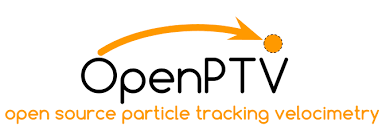
\includegraphics[width=0.5\textwidth]{openptv_logo} \hspace{1em} library, `liboptv`, ANSI C
\item PyPTV GUI for {\em liboptv} in Python 
\includegraphics[width=.3\textwidth]{pyptv}
\item FlowTracks - trajectories database management (see Meller and Liberzon 2016)
\item BlobRecorder - proprietary hardware/customized software (see Shnapp et al. arxiv)
\end{frame}



\section{Results}\label{sec:results}
\subsubsection*{Trajectory Dataset}
%
\begin{frame}
	\centering
	\cardImg{traj_snapshot3.pdf}{1\textwidth}
%\begin{card} A visualization of Lagrangian trajectories at various heights in the canopy model. A view from the bottom wall.
%\end{card}
\end{frame}


\begin{frame}{PDF of tracking times}
\centering \cardImg{PDF_of_Tracking_time_25.png}{0.8\textwidth}
\begin{cardTiny} Tracking time of trajectories, $t_\text{tr}$, from different heights for the  $Re_\infty=16\times10^3$ case. \end{cardTiny} 
\end{frame}


\subsubsection*{Velocity Distributions}
\begin{frame}
	\centering
	\cardImg{vx_PDF_U40.png}{0.9\textwidth}
	\vspace{-.3cm}
	\begin{cardTiny} PDF of the $u_x/U_\infty$ at 5 height bins inside and above the canopy height $H$ for the $Re_\infty = 26\times 10^3$ case. 
	\end{cardTiny}
\end{frame}


\subsubsection*{Lagrangian Accelerations}

\begin{frame}
\centering\cardImg{ax_pdf_U40.png}{.9\textwidth}
\begin{cardTiny} %$Re_\infty=26\times 10^3$ case from 5 bin-heights.
\begin{equation}
P(a) = C \exp \left[- \frac{a^2}{\left( 1 + |a\beta / \sigma|^\gamma   \right) \sigma^2} \right]
\label{eq:stretched_exp}
\end{equation}
with $\beta=\sigma=0.57$, $\gamma=1.5$ and $C = 0.686$. 
\end{cardTiny}
\end{frame}


\begin{frame}
\centering\cardImg{accel_variance.png}{.9\textwidth}
\begin{cardTiny} $\langle a_x^2 \rangle^{1/2}$, normalized with the $u'$ and $H$.\end{cardTiny}
%
\end{frame}


%\section*{Possible extensions}
%\begin{frame}{What can we do to increase 3D-PTV usability}
%\begin{multicols}{2}
%% \cardImg{calibration1}{.32\textwidth}
%\cardImg{dumbbell1}{.49\textwidth}
%\cardImg{dumbbell2}{.49\textwidth}
%\end{multicols}
%\end{frame}



%\begin{frame}{Single camera - multiple views}
%\centering\cardImg{ldc_splitter}{0.8\textwidth}
%% \begin{cardTiny} A high speed camera with a four-view optical system \end{cardTiny}
%\end{frame}

%\begin{frame}{3D-PTV can slide or rotate}
%\begin{columns}
%\column{6cm}
%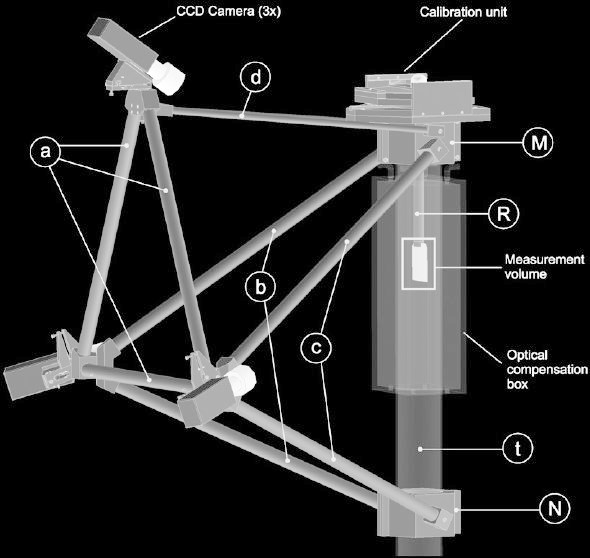
\includegraphics[width=.9\textwidth]{sliding_ptv.png}\\
%{\scriptsize Walpot et al. Meas. Sci. Tech. 2006. TU/e} 
%
%\column{6cm}
%\movie[label=show3,width=0.8\textwidth,poster
%       ,autostart,showcontrols,loop] 
%  {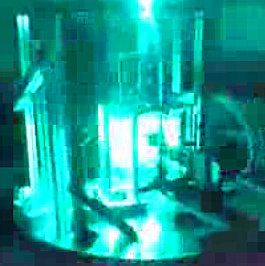
\includegraphics[width=0.8\textwidth]{rotation.png}}{rotation.mov}
%\end{columns}
%\end{frame}




\section{Summary and conclusions}\label{sec:summary}

\begin{frame}{Summary}
\begin{itemize}
\item Real time imaging changed the 3D-PTV method and the way we think about it
\item Field experiments, webcam or Kinect-based, wind tunnel experiments, space station microgravity experiments are possible
\item Direct Lagrangian information in complex urban canopy flows is under analysis
\item Close coordination with the modeling efforts of Lagrangian dispersion or Lagrangian puff models
\end{itemize}
\end{frame}

\begin{frame}{Thank you for your attention}
\cardImg{photo}{\textwidth}
\end{frame}

\end{document}














